\documentclass[aspectratio=169, 11pt]{beamer}
% ============================================================================
%  23CSE498 -- Project Phase 2, Panel Review 1
%  Structural Descriptors for Metal-Organic Frameworks
%  Compile:  pdflatex panel_review.tex   (twice, for the section numbering)
%  Note: \bibliography is commented out -- references are typeset directly so
%        the deck compiles without needing a bibtex pass. Uncomment if wanted.
% ============================================================================
\usepackage[utf8]{inputenc}
\usepackage[T1]{fontenc}
\usepackage{xcolor}
\usepackage{booktabs}
\usepackage{graphicx}
\usepackage{amsmath}
\usepackage{tikz}
\usetikzlibrary{calc, arrows.meta, positioning}
\graphicspath{{../}{./}{../4_reference/}}
\IfFileExists{opensans.sty}{\usepackage[default,scale=0.95]{opensans}}{}

% --- Branding ---
\definecolor{amritaMaroon}{HTML}{A4123F}
\definecolor{okGreen}{HTML}{0D6B47}
\definecolor{warnRed}{HTML}{B02A2A}
\definecolor{coolBlue}{HTML}{1F5FA8}
\definecolor{softGrey}{HTML}{F4F6FA}

\usetheme{Madrid}
\usecolortheme[named=amritaMaroon]{structure}
\setbeamertemplate{navigation symbols}{}
\setbeamertemplate{footline}[frame number]
\setbeamertemplate{itemize items}[circle]
\setbeamerfont{block title}{size=\small}

\begin{document}

% ============================ TITLE ==========================================
\begin{frame}
    \begin{tikzpicture}[remember picture,overlay]
        \node[fill=amritaMaroon, text=white, font=\bfseries\footnotesize,
              anchor=north east, rounded corners=2pt, inner sep=5pt]
        at ($(current page.north east) + (-0.2cm,-0.2cm)$)
        {Type 1: Research Project};
    \end{tikzpicture}
    \centering
    \IfFileExists{logo.png}{\includegraphics[width=2.4cm]{logo.png}}{\vspace{1.2cm}}
    \vspace{0.05cm}

    {\large \textbf{\textcolor{amritaMaroon}{Structural Descriptors for Metal--Organic
    Frameworks:}}}\\
    {\normalsize \textbf{\textcolor{amritaMaroon}{Multifractal Analysis of Framework
    Connectivity for Simulation-Free Screening}}} \\
    \vspace{0.05cm}
    {\footnotesize \textbf{23CSE498 -- Project Phase 2 (Panel Review 1)} \quad | \quad
     \textbf{Team Number: [XX]}} \\
    \vspace{0.1cm}

    \begin{table}
        \centering
        \scriptsize
        \renewcommand{\arraystretch}{1.05}
        \begin{tabular}{|c|c|l|}
            \hline
            \textbf{S.No} & \textbf{Register Number} & \textbf{Student Name} \\
            \hline
            1 & CB.SC.U4CSE23134 & P. M. Radha Krishna \\
            \hline
            2 & CB.SC.U4CSE23122 & P. Kshitij Varma \\
            \hline
            3 & CB.SC.U4CSE23141 & G. Rohith Abhinav \\
            \hline
            4 & CB.SC.U4CSE23031 & J. Keerthi Sree \\
            \hline
            5 & CB.SC.U4CSE23029 & Isha Sri Prakash \\
            \hline
        \end{tabular}
    \end{table}
    \vspace{0.05cm}

    {\footnotesize Guide: \textbf{Dr.~T.~Ramraj}, M.E, Ph.D --- Assistant Professor (Sl.\,Gd.),}\\
    {\footnotesize Department of Computer Science and Engineering, School of Computing, Coimbatore} \\
    \vspace{0.05cm}
    {\scriptsize \today}
\end{frame}

% ============================ PROBLEM CONTEXT ================================
\section{Problem Context}
\begin{frame}{0. Problem Context --- Why This Project Exists}
\framesubtitle{The gap between the number of candidate materials and our ability to evaluate them}
\begin{columns}[T]
\column{0.54\textwidth}
\textbf{The materials-science problem}
\begin{itemize}\footnotesize
  \item \textbf{Metal--organic frameworks (MOFs)} are crystalline solids built by joining
        metal clusters (\textit{nodes}) to organic molecules (\textit{linkers}).
  \item They are extremely porous --- internal surface areas above
        3{,}000\,m$^2$/g --- making them candidates for gas storage, carbon capture and
        separation.
  \item \textbf{Hundreds of thousands} of MOFs are known or hypothesised.
\end{itemize}

\vspace{0.15cm}
\textbf{The computational bottleneck}
\begin{itemize}\footnotesize
  \item Evaluating one MOF by molecular simulation (GCMC) takes \textbf{hours}.
  \item Exhaustive screening of the design space is \textbf{not feasible}.
\end{itemize}

\column{0.46\textwidth}
\begin{block}{\footnotesize Research Question}
\footnotesize
Can a \textbf{purely structural, simulation-free descriptor} --- computed from a framework's
\textit{connectivity} in seconds --- group MOFs into meaningful families, so a new candidate
can be triaged \textbf{without} expensive calculation?
\end{block}

\vspace{0.1cm}
\begin{block}{\footnotesize Value Proposition}
\footnotesize
Not a \textit{replacement} for simulation --- a \textbf{filter} that decides
\textbf{what to simulate}. Reducing $10^5$ candidates to $10^2$ is the contribution.
\end{block}
\end{columns}
\end{frame}

% ============================ SLIDE 1: METHODOLOGY ===========================
\section{Methodology \& Solution Design}
\begin{frame}{1. Methodology \& Solution Design}
\framesubtitle{Rubric: Workflow, Architecture, Algorithms/Mathematical Model \& Evaluation Metrics (5 Marks)}
\begin{columns}[T]
\column{0.46\textwidth}
{\scriptsize
\textbf{Theoretical foundation.} A MOF is a \textbf{periodic graph}. Collapse each building
block to a vertex and each inter-block bond to an edge; the chemistry reduces to pure
connectivity, which the properties follow.

\vspace{0.12cm}
\textbf{Core algorithms}
\begin{itemize}\scriptsize
  \item \textbf{Decomposition:} MOFid metal-oxo algorithm~[1] --- PBC-aware bond
        perception, connected-component block extraction.
  \item \textbf{Graph construction:} \textit{labelled quotient graph} --- edges carry a
        lattice translation $t$, so the infinite crystal is represented exactly.
  \item \textbf{Descriptor:} influential-node multifractal analysis (iNMFA)~[2].
\end{itemize}

\vspace{0.12cm}
\textbf{Dataset.} \textbf{138 frameworks}: 77 hypothetical (hMOF, via MOFX-DB~[7]) and 61
experimentally synthesised (CoRE MOF 2019, via its Zenodo DOI), both with published PLD/LCD
pore diameters. Supercells of 1{,}160--7{,}000 atoms.
}

\column{0.54\textwidth}
\centering
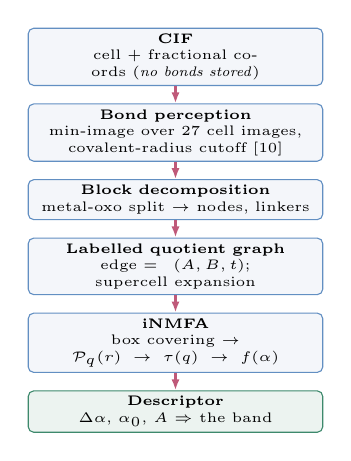
\begin{tikzpicture}[
  node distance=0.22cm,
  every node/.style={font=\tiny},
  box/.style={draw=coolBlue!70, fill=softGrey, rounded corners=2pt,
              text width=3.6cm, align=center, inner sep=2pt, minimum height=0.40cm},
  outbox/.style={draw=okGreen!80, fill=okGreen!8, rounded corners=2pt,
              text width=3.6cm, align=center, inner sep=2pt, minimum height=0.40cm},
  ar/.style={-{Latex[length=1.4mm]}, draw=amritaMaroon!70, thick}]
  \node[box] (a) {\textbf{CIF} \\ cell + fractional coords (\textit{no bonds stored})};
  \node[box, below=of a] (b) {\textbf{Bond perception} \\ min-image over 27 cell images,
                              covalent-radius cutoff~[10]};
  \node[box, below=of b] (c) {\textbf{Block decomposition} \\ metal-oxo split $\to$ nodes,
                              linkers};
  \node[box, below=of c] (d) {\textbf{Labelled quotient graph} \\ edge $=(A,B,t)$;
                              supercell expansion};
  \node[box, below=of d] (e) {\textbf{iNMFA} \\ box covering $\to \mathcal{P}_q(r) \to
                              \tau(q) \to f(\alpha)$};
  \node[outbox, below=of e] (f) {\textbf{Descriptor} \\ $\Delta\alpha$, $\alpha_0$, $A$
                                 $\Rightarrow$ the band};
  \draw[ar] (a)--(b); \draw[ar] (b)--(c); \draw[ar] (c)--(d);
  \draw[ar] (d)--(e); \draw[ar] (e)--(f);
\end{tikzpicture}

\vspace{0.05cm}
{\tiny \textbf{Validation metric:} published \textbf{coordination numbers} --- an
independent ground truth the graph must reproduce.}
\end{columns}
\end{frame}

% ============================ SLIDE 1b: MATH =================================
\begin{frame}{1b. Mathematical Model}
\framesubtitle{The descriptor, defined}
\begin{columns}[T]
\column{0.52\textwidth}
{\scriptsize
\textbf{Step 1 --- the measure.} For each influential node $i$ (top 10\% by degree) and box
radius $r$, let $M_i(r)$ be the number of vertices within $r$ steps:
\vspace{-0.15cm}
\[ p_i(r) = M_i(r)/N \]
\vspace{-0.45cm}

\textbf{Step 2 --- the partition function}, reweighted by a distortion factor $q$:
\vspace{-0.15cm}
\[ \mathcal{P}_q(r) = \sum_{i \in I} p_i(r)^{\,q} \]
\vspace{-0.45cm}

\textbf{Step 3 --- the mass exponent.}
\vspace{-0.15cm}
\[ \boxed{\ \tau(q) = \frac{\ln \mathcal{P}_q(r)}{\ln (r/r_N)}\ } \]
\vspace{-0.45cm}

\textbf{Step 4 --- Legendre transform.}
\vspace{-0.15cm}
\[ \alpha(q) = \frac{d\tau}{dq}, \quad f(\alpha) = q\,\alpha(q) - \tau(q) \]
}

\column{0.48\textwidth}
\begin{block}{\footnotesize Interpreting the spectrum}
{\tiny
\begin{tabular}{@{}ll@{}}
\toprule
\textbf{Quantity} & \textbf{Physical meaning} \\
\midrule
$\alpha$ & local growth rate around one block \\
$f(\alpha)$ & how much of the framework shares it \\
$\alpha_0$ & the \textit{typical} dimension (apex) \\
$\Delta\alpha$ & \textbf{heterogeneity} of the pore network \\
$A$ & asymmetry --- dense-vs-open dominance \\
\bottomrule
\end{tabular}}
\end{block}

\vspace{0.05cm}
\begin{block}{\footnotesize Structural constraint used as a correctness test}
\tiny
$f(\alpha)$ \textbf{must} be an inverted parabola peaking at $q=0$, where
$f(\alpha_0)=D_0$. \textbf{Any implementation not producing this shape is wrong} --- we
used it as a test, and it caught a real defect (Slide 3).
\end{block}

\vspace{0.05cm}
{\tiny \textbf{Evaluation metrics:} coordination-number agreement with published
crystallography; spectrum shape (\% peaking at $q=0$); seed reproducibility; partial
correlation against pore diameter.}
\end{columns}
\end{frame}

% ============================ SLIDE 2: IMPLEMENTATION ========================
\section{Implementation Progress}
\begin{frame}{2. Implementation Progress \& Module Functionality}
\framesubtitle{Rubric: Core Modules Implemented, Functional \& Integrated (8 Marks)}
\vspace{-0.32cm}
\begin{table}
\centering
\tiny
\renewcommand{\arraystretch}{0.99}
\begin{tabular}{p{3.0cm} p{7.0cm} c}
\toprule
\textbf{Module / Component} & \textbf{Current Implementation State} & \textbf{Status} \\
\midrule
Data ingestion (\texttt{code\_01--02}) & CIF parsing, symmetry expansion, PBC bond
perception over 27 cell images & \textcolor{okGreen}{\textbf{Functional}} \\
Decomposition (\texttt{code\_03--04}) & \texttt{is\_metal()} classification; metal-oxo,
single-node, all-node splits & \textcolor{okGreen}{\textbf{Functional}} \\
Topology export (\texttt{code\_05--07}) & Centroid simplification, Systre \texttt{.cgd}
writer, MOFid/MOFkey assembly & \textcolor{okGreen}{\textbf{Functional}} \\
Network analysis (\texttt{code\_09}) & Labelled quotient graph, degree/eigenvector/
betweenness centrality, Laplacian & \textcolor{okGreen}{\textbf{Functional}} \\
Spectrum (\texttt{code\_10--11}) & iNMFA (box-covering) and NMFA (box-growing);
$\tau$, $\alpha$, $f(\alpha)$, $\Delta\alpha$, $A$ & \textcolor{okGreen}{\textbf{Functional}} \\
77-framework study & Live MOFX-DB query, spectra for all 77, band + confound analysis &
\textcolor{okGreen}{\textbf{Functional}} \\
Interactive web platform & 9-page documentation portal; full pipeline runs live in-browser
on any uploaded CIF; 5 headless test suites gate publication &
\textcolor{okGreen}{\textbf{Integrated}} \\
Size-matched comparison & 61 synthesised MOFs expanded under the identical 48\,\AA{} rule
and compared against the 77 & \textcolor{okGreen}{\textbf{Functional}} \\
Dataset release & 138 frameworks, CC BY 4.0, with schema, provenance and both withdrawn
claims documented & \textcolor{okGreen}{\textbf{Functional}} \\
Experimental-set validation at scale & \textbf{Done:} 61 CoRE MOF frameworks via Zenodo DOI,
no API dependency & \textcolor{okGreen}{\textbf{Functional}} \\
\bottomrule
\end{tabular}
\end{table}
\vspace{-0.32cm}
{\tiny
\textbf{Two axes, because ``built'' and ``established'' are different claims.}
\textbf{Engineering $\approx$96\%}: 14 Python modules, an independent browser
implementation that cross-checks them, a 10-page platform, 6 CI-gating test suites, the
138-framework study end to end, a released dataset.
\textbf{Validation $\approx$73\%}: the descriptor is provably correct, its failure modes are
documented, and it now \textbf{transfers to experimentally synthesised structures} --- 61 of
them, size-matched. Not established: that $\Delta\alpha$ predicts any measured property.
The two engines are also not yet reconciled at supercell size.
\textbf{Weighted $\approx$85\%} (rubric asks $\approx$60\%).
\textbf{Verification:} Python and JavaScript agree at unit-cell size ($\tau(0)=-2.6551$,
HKUST-1). \textbf{github.com/Radha-Krishna-19/fyp}}
\end{frame}

% ============================ SLIDE 2b: RESULTS ==============================
\begin{frame}{2b. Results Obtained So Far}
\framesubtitle{Every number computed from the live pipeline --- nothing transcribed}
\begin{columns}[T]
\column{0.5\textwidth}
\begin{block}{\footnotesize Validation --- the graph is correct}
{\scriptsize
\begin{tabular}{@{}lccc@{}}
\toprule
& \textbf{Node c.n.} & \textbf{Published} & \textbf{Net} \\
\midrule
HKUST-1 & 4 & (4,\,3) & \texttt{tbo} \\
MOF-5 & 6 & (6,\,2) & \texttt{pcu} \\
ZIF-8 & 4 & (4,\,2) & \texttt{sod} \\
UiO-66 & \textbf{12} & (12,\,2) & \texttt{fcu} \\
\bottomrule
\end{tabular}
\vspace{0.1cm}

All four match. A naive construction gives UiO-66 = \textbf{1}.}
\end{block}

\begin{block}{\footnotesize Defects make influence measurable}
{\scriptsize
In a perfect crystal every block is symmetry-equivalent $\Rightarrow$ only \textbf{2}
distinct centrality values $\Rightarrow$ ``top-$k$'' is a \textbf{tie}.
Remove one linker: $2 \to 4$ distinct values, and
$\lambda_2: 1.44 \to 1.19$ --- the weakening, quantified.}
\end{block}

\column{0.5\textwidth}
\begin{block}{\footnotesize The band, as originally measured}
{\scriptsize
\begin{tabular}{@{}lcc@{}}
\toprule
& \textbf{Hypothetical} & \textbf{Synthesised} \\
& 77 hMOF & 61 CoRE MOF \\
\midrule
Valid spectra & 77 / 77 & 61 / 61 \\
$\Delta\alpha$ range & 1.02 -- 1.41 & 0.95 -- 1.47 \\
Mean $\Delta\alpha$ & 1.180 & \textbf{1.198} \\
Mean asymmetry $A$ & $-1.31$ & \textbf{$-1.31$} \\
\bottomrule
\end{tabular}
\vspace{0.1cm}

Means differ by \textbf{0.018} (Welch $p=0.38$). Same shape on both sets ---
but \textbf{withdrawn}, see slide 3f: computed on the wrong graph, and shown
not to converge on the right one either.}
\end{block}

\begin{alertblock}{\footnotesize What the band does \textit{not} mean}
{\scriptsize
\begin{tabular}{@{}lr@{}}
$\Delta\alpha$ vs pore diameter, raw & $-0.497$ \\
\quad controlling for graph size & \textbf{$+0.101$} \\
$\Delta\alpha$ vs graph size, ctrl.\ pore & \textbf{$+0.621$} \\
\midrule
$R^2$: size alone / +pore & 0.533 / 0.538 \\
\end{tabular}
\vspace{0.08cm}

Pore size adds \textbf{+0.005}. This confound is now understood as one
symptom of a larger problem, not a standalone finding --- \textbf{see slides
3f--3g}.}
\end{alertblock}
\end{columns}
\end{frame}

% ============================ SLIDE 3: TECHNICAL KNOWLEDGE ===================
\section{Technical Knowledge}
\begin{frame}{3. Technical Knowledge \& Design Decisions}
\framesubtitle{Rubric: Understanding of Methodology, Implementation \& Design Choices (5 Marks)}
\begin{columns}[T]
\column{0.5\textwidth}
{\scriptsize
\textbf{Why a graph representation?} MOF properties follow \textit{connectivity}: gas moves
through the pore network, and the pore network is the void left by the wiring. An
\textbf{unweighted} graph deliberately discards element identity --- what survives is
\textbf{pure architecture}, which transfers across chemistries.

\vspace{0.1cm}
\textbf{Key design decisions}
\begin{itemize}\scriptsize
  \item \textbf{Labelled quotient graph over a naive graph.} Without translation labels,
        UiO-66's 12-connected cluster reports as \textbf{1} --- or degenerates into a star.
  \item \textbf{Supercell expansion.} A primitive cell has diameter $\sim$2, too small for
        a power-law fit. Expansion is \textit{exact} because edges carry translations.
  \item \textbf{Box-growing (deterministic) validated against box-covering (stochastic).}
  \item \textbf{Defect simulation} to break symmetry --- physically justified by~[15].
\end{itemize}
}

\column{0.5\textwidth}
\begin{alertblock}{\footnotesize Defect found by our own shape test}
{\scriptsize
The spectra were not parabolic. Cause: $\tau(q)$ was extracted with a
\textbf{free-intercept} least-squares slope, but~[2] defines it as a \textbf{ratio}
$\ln\mathcal{P}_q/\ln(r/r_N)$ --- a fit \textbf{through the origin}.

At $q=0$: every term is $p_i^0=1$, so $\mathcal{P}_0=|I|$ is \textbf{constant in $r$}.
A flat line has slope $0 \Rightarrow \tau(0)=0 \Rightarrow f(\alpha_0)=0$ ---
\textbf{the peak is deleted}.
\vspace{0.08cm}

\begin{tabular}{@{}lccc@{}}
\toprule
$\tau$ definition & $\tau(0)$ & $f(\alpha_0)$ & parabola \\
\midrule
free intercept & 0.0000 & 0.0000 & \textcolor{warnRed}{no} \\
\textbf{paper (ratio)} & $-2.5669$ & $+2.5669$ & \textcolor{okGreen}{\textbf{yes}} \\
\bottomrule
\end{tabular}}
\end{alertblock}

{\tiny
\textbf{Trade-offs.} \texttt{MIN\_CELL\_LENGTH}/\texttt{MAX\_ATOMS} trade scaling range
against $O(N^2)$ memory --- and are the source of the size confound we identified.
\textbf{Influential-node selection is ambiguous in a perfect crystal} (all degrees tie);
we report the ambiguity rather than hide it.}
\end{columns}
\end{frame}

% ============================ SLIDE 3b: PLATFORM =============================
\begin{frame}{3b. Deliverable --- Interactive Analysis Platform}
\framesubtitle{An 18-section technical site; the full pipeline executes in-browser}
{\footnotesize
\begin{columns}[T]
\column{0.5\textwidth}
\textbf{What it does}
\begin{itemize}\scriptsize
  \item Runs the \textbf{complete decomposition live} on any uploaded \texttt{.cif} ---
        no server, no installation.
  \item Steps through all nine pipeline modules with the \textbf{real source code beside a
        live 3D model} of the structure at that stage.
  \item Computes the network analysis and the multifractal spectrum \textbf{in the browser},
        cross-validated against the Python reference.
\end{itemize}
\column{0.5\textwidth}
\textbf{Built for a mixed audience}
\begin{itemize}\scriptsize
  \item A \textbf{graph-theory primer} (Section 10) defines every term --- vertex, degree,
        quotient graph, Laplacian, $\lambda_2$, defect --- \textit{before} it is used.
  \item Every source file is readable by clicking its name anywhere on the page.
  \item Automated test suites cover the decomposition, the network layer, the band analysis
        and the site structure itself.
\end{itemize}
\end{columns}}
\end{frame}

% ---- the main result, full width so it is legible ----
\begin{frame}{3c. Principal Result --- All 77 Spectra and the Band}
\framesubtitle{Computed live from the pipeline; nothing transcribed}
\centering
\IfFileExists{band77_figure.png}{%
  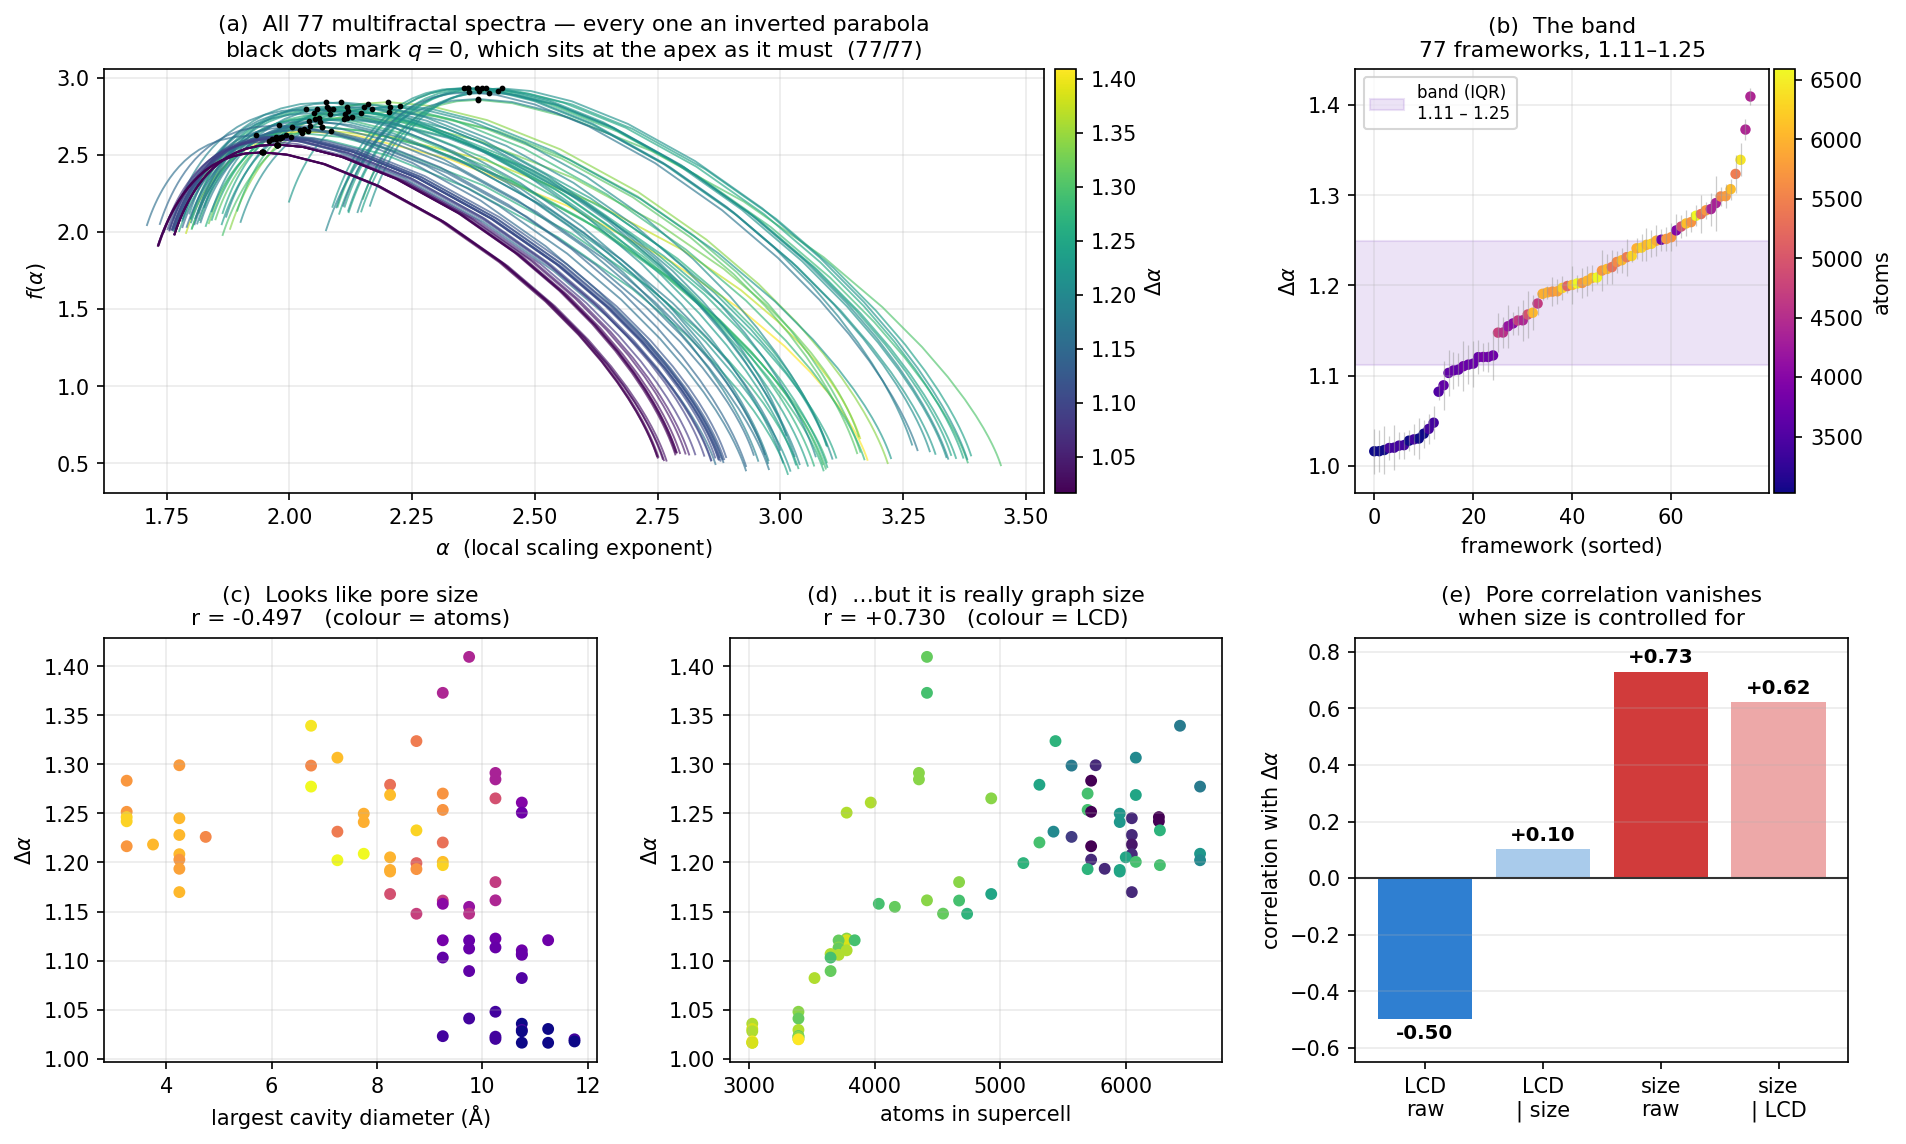
\includegraphics[width=0.99\linewidth,height=0.68\textheight,keepaspectratio]{band77_figure.png}%
}{%
  \fbox{\begin{minipage}{10cm}\centering\vspace{2cm}
  \textbf{[band77\_figure.png]}\vspace{2cm}\end{minipage}}
}

\vspace{-0.15cm}
{\tiny \textbf{(a)} all 77 spectra are proper inverted parabolas, $q=0$ at the apex \quad
\textbf{(b)} a tight band, $\Delta\alpha=1.11$--$1.25$ \quad \textbf{(c--e)} the apparent
pore correlation ($-0.50$) collapses to $+0.10$ controlling for graph size; size survives at
$+0.62$.}
\end{frame}

% ---- the transfer result, and the claim we withdrew to get it ----
\begin{frame}{3d. Does It Transfer? 61 Frameworks That Actually Exist}
\framesubtitle{The band was calibrated on structures nobody has ever made}
\centering
\IfFileExists{fig09_real_vs_hmof.png}{%
  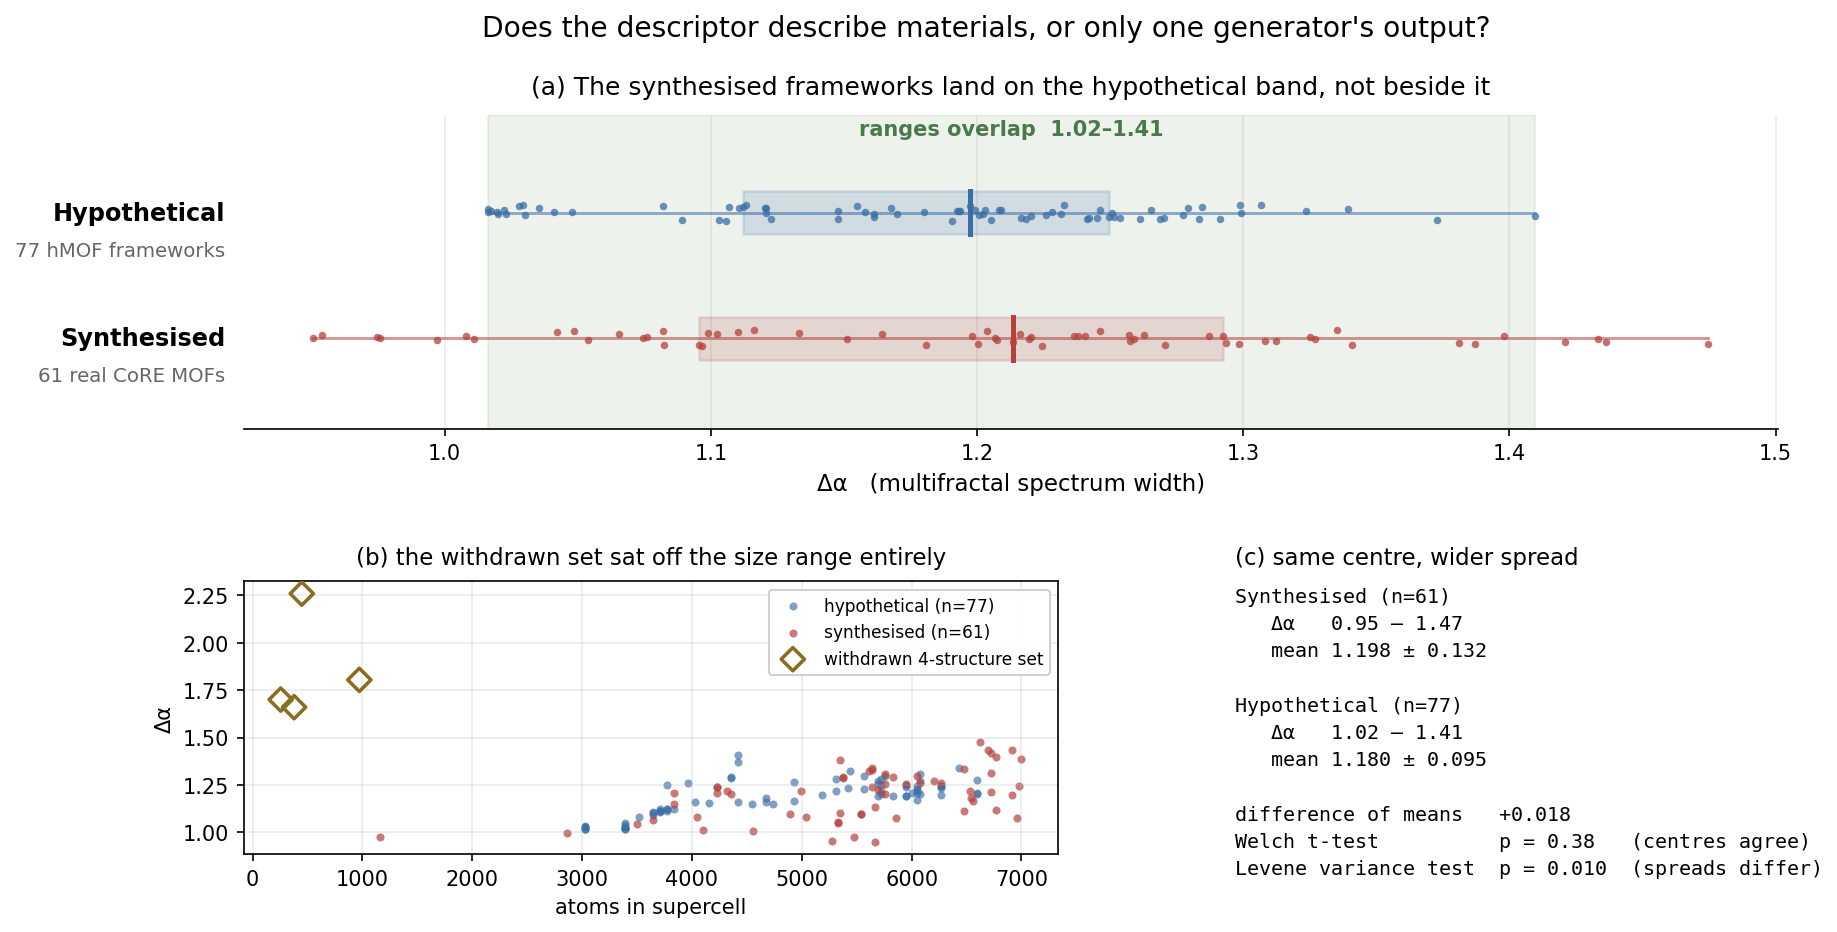
\includegraphics[width=0.99\linewidth,height=0.62\textheight,keepaspectratio]{fig09_real_vs_hmof.png}%
}{%
  \fbox{\begin{minipage}{10cm}\centering\vspace{2cm}
  \textbf{[fig09\_real\_vs\_hmof.png]}\vspace{2cm}\end{minipage}}
}

\vspace{-0.1cm}
{\tiny \textbf{(a)} 61 synthesised frameworks land \textit{on} the hypothetical band:
$0.95$--$1.47$ vs $1.02$--$1.41$, means differing by $0.018$ (Welch $p=0.38$).
\textbf{(b)} \textcolor{warnRed}{\textbf{We withdrew our own result to get here.}} The four
MOFs we previously reported at $1.66$--$2.26$ are the gold diamonds --- 256--972 atoms,
off the size range of both clouds. $\Delta\alpha$ rises with atom count ($r=+0.73$), so that
comparison measured graph size. \textbf{(c)} Same centre; the real set is significantly
\textit{more} variable (Levene $p=0.010$).}
\end{frame}

% ---- the confound analysis, reproduced on real materials ----
\begin{frame}{3e. The Same Confound Analysis, Redone on Real Materials}
\framesubtitle{If a result is real it should survive being asked twice, of different material}
\centering
\IfFileExists{fig10_real_band61.png}{%
  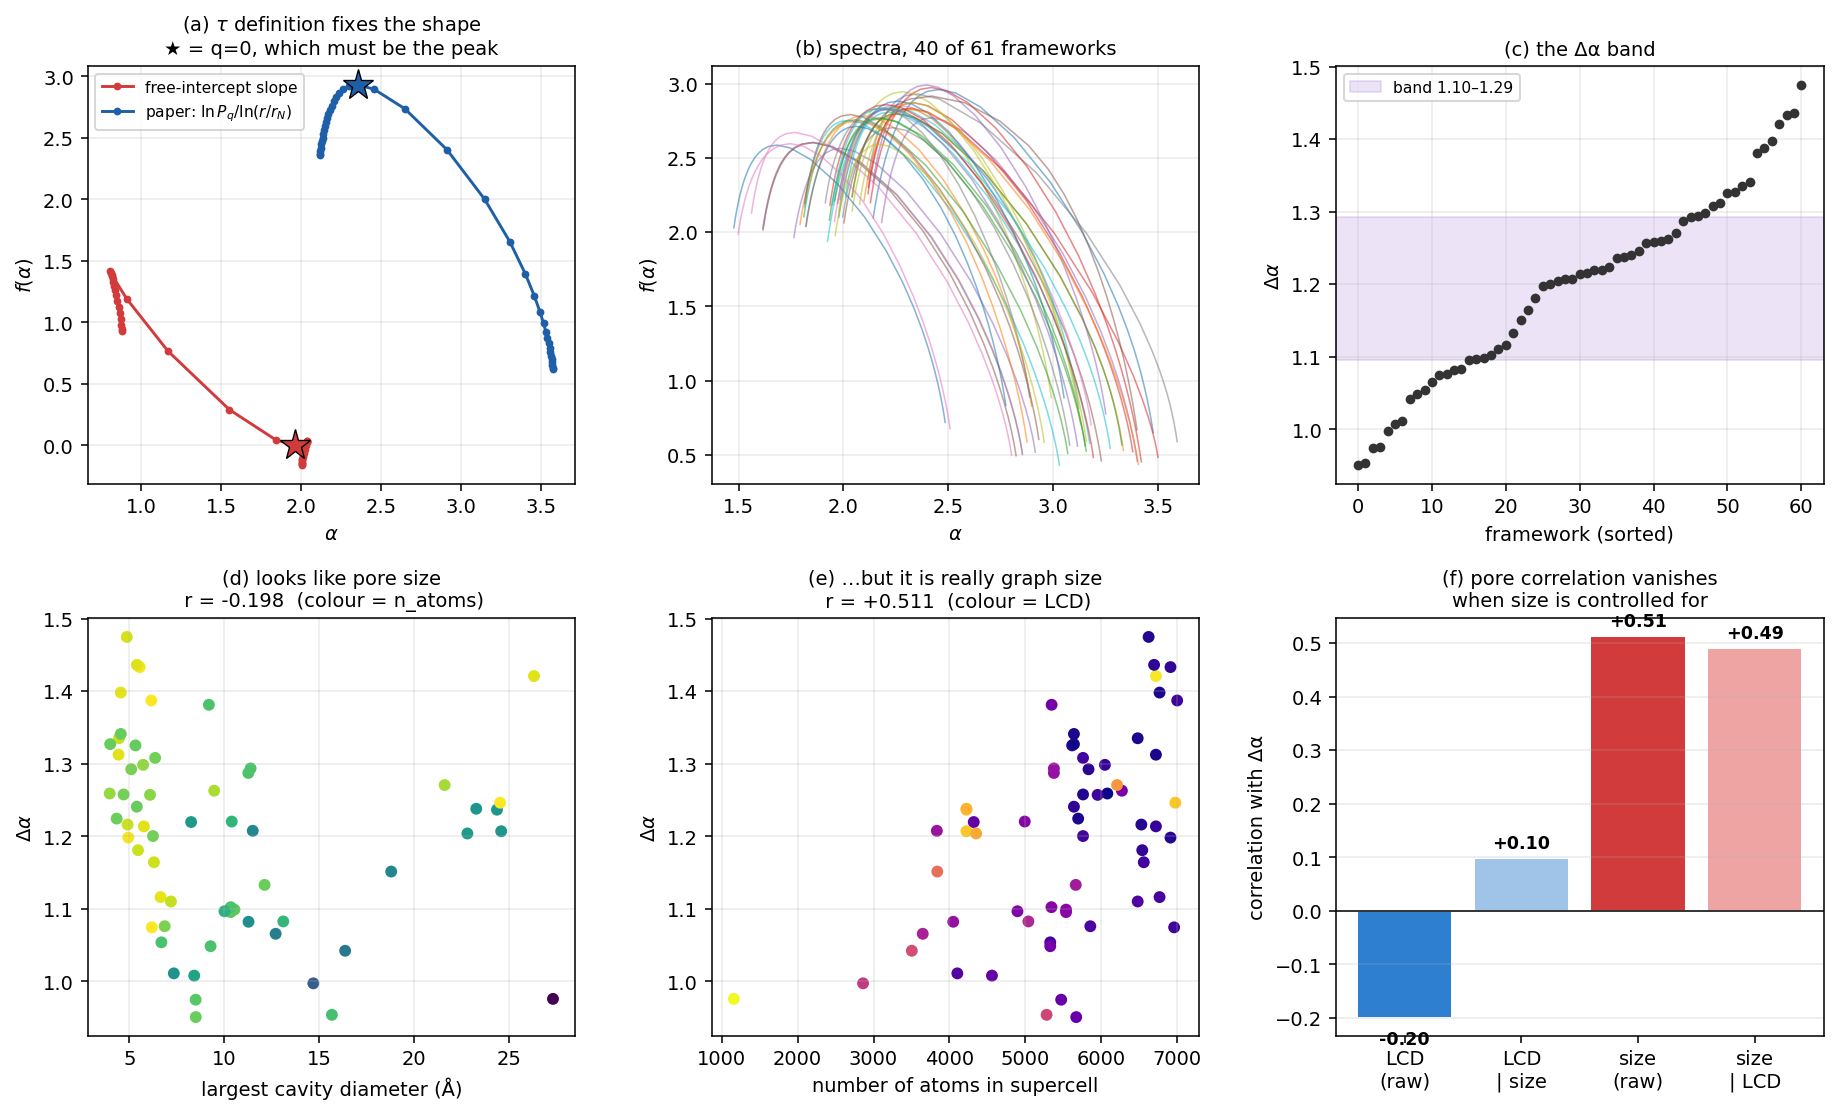
\includegraphics[width=0.99\linewidth,height=0.62\textheight,keepaspectratio]{fig10_real_band61.png}%
}{%
  \fbox{\begin{minipage}{10cm}\centering\vspace{2cm}
  \textbf{[fig10\_real\_band61.png]}\vspace{2cm}\end{minipage}}
}

\vspace{-0.1cm}
{\tiny \textbf{(a)} why the $\tau$ definition matters: free-intercept (red) is not a spectrum;
through-origin (blue) is, with $q=0$ at the apex. \quad
\textbf{(b--c)} 61 real spectra and their band, $1.10$--$1.29$ --- against $1.11$--$1.25$ for
the 77 hypothetical. \quad
\textbf{(d--f)} \textcolor{okGreen}{\textbf{the pore-size confound reproduces exactly.}}
Raw $\Delta\alpha$--LCD correlation $-0.20$; hold graph size constant and it collapses to
$+0.10$, while size survives at $+0.49$. The claim we withdrew on hypothetical structures fails
the same way, for the same reason, on structures that exist --- which is the strongest evidence
we have that the confound analysis was right rather than a quirk of one dataset.}
\end{frame}

% ---- 3f: the negative result that supersedes 3c/3d/3e above -----------------
\begin{frame}{3f. Both Bands Above Are Withdrawn}
\framesubtitle{A finite-size test run after slides 3c--3e were written, 2026-09-14/15}
\begin{block}{\footnotesize The band does not converge with supercell size}
\scriptsize
$\Delta\alpha$ was measured over $q\in[-10,10]$; at extreme $q$ a single box (as small as one
vertex) dominates the sum, so $\Delta\alpha$ inherits a term that grows with graph size without
bound. Fitted slope of $\Delta\alpha$ vs $\ln(\text{diameter})$, full $q$ range, on the
\textit{correct} coarse-grained graph, four nets: HKUST-1 (tbo) 0.782, MOF-5 (pcu) 0.732,
ZIF-8 (sod) 0.886, UiO-66 (fcu) 0.692 --- all $R^2 \geq 0.998$. Tested at six caps on $|q|$
(10, 8, 5, 4, 3, 2): \textbf{none converged} on any net.
\end{block}
\begin{block}{\footnotesize Both published bands were also measured on the wrong graph}
\scriptsize
Both the 77-framework and 61-framework bands in slides 3c--3e were computed on the
\textbf{atomic} supercell graph, not the coarse-grained building-block graph this project's
method describes. An atomic graph spans a molecular length scale and a framework length scale;
fitting one power law across that crossover is invalid independently of the finite-size problem
above.
\end{block}
\begin{block}{\footnotesize What this means for slides 3c--3e}
\scriptsize
None of the three is a structural or chemical finding. All are kept, with this notice, for
audit --- the same treatment given to the pore-size and four-structure withdrawals already on
this deck. The +0.62 correlation with graph size in 3c was not a confound contaminating the
descriptor: it \textbf{was} the descriptor. See \texttt{CLAUDE.md} and the project Results page.
\end{block}
\end{frame}

% ---- 3g: redone correctly, on the complete datasets --------------------------
\begin{frame}{3g. Redone Correctly, on the Complete Datasets}
\framesubtitle{All 77 hMOF, all 61 CoRE MOF, on the coarse-grained supercell graph this time}
\begin{columns}[T]
\column{0.5\textwidth}
\begin{block}{\footnotesize What ran}
\scriptsize
Both datasets re-fetched in full and re-analysed on the graph the method actually specifies.
72/77 hMOF and 55/61 CoRE MOF produced a usable spectrum (the rest fell below the diameter-8
scaling gate). One spectrum per structure, one seed --- no per-structure error bar to check
classes against, stated as a limitation, not hidden.
\end{block}
\begin{block}{\footnotesize The result does not change}
\scriptsize
Sorted into Narrow/Medium/Wide by $\Delta\alpha$ (same rule as before), class correlates with
coarse-grained node count at $\mathbf{r=+0.70}$ on \textbf{both} datasets, independently.
\textbf{Using the right graph fixes the graph. It does not fix the descriptor.}
\end{block}
\column{0.5\textwidth}
\begin{block}{\footnotesize Nine-category check, per class}
\scriptsize
Chemistry, graph features, degree, edges, clustering, assortativity, heterogeneity, components
--- checked per class, both datasets. hMOF: Narrow and Medium (65/72) are the \textbf{same
graph} in every category except width --- same metal, same net, same block count, same
assortativity to 3 decimals. CoRE MOF: classes differ on chemistry and graph size at once,
always in the same direction, so this cannot separate which one is doing the separating.
\end{block}
\begin{alertblock}{\footnotesize A new, undocumented finding along the way}
\scriptsize
Several classes on both datasets average $>1$ connected component after replication, which
should always be exactly 1. The metal-oxo decomposition is retaining disconnected
guest/solvent fragments as small ``linker'' blocks on a real fraction of structures --- worth
its own follow-up.
\end{alertblock}
\end{columns}
\end{frame}

% ============================ SLIDE 4: MOOC ==================================
\section{Technical Enrichment}
\begin{frame}{4. Technical Enrichment Activity Choices}
\framesubtitle{Professional Online Certification Details (Individual Mandatory: 10--20 Hours)}
\vspace{-0.1cm}
\begin{table}
\centering
\scriptsize
\renewcommand{\arraystretch}{1.12}
\begin{tabular}{|c|p{2.6cm}|p{4.6cm}|p{2.0cm}|c|}
\hline
\textbf{S.No} & \textbf{Student Name} & \textbf{Chosen MOOC / Course Title} &
\textbf{Platform} & \textbf{Hours} \\
\hline
1 & P. M. Radha Krishna & Algorithms on Graphs (BFS, shortest paths, connected
components) & Coursera (UC San Diego) & 20 Hrs \\
\hline
2 & P. Kshitij Varma & Introduction to Complex Network Analysis &
NPTEL & 20 Hrs \\
\hline
3 & G. Rohith Abhinav & Chemoinformatics / Computational Materials Science &
NPTEL & 16 Hrs \\
\hline
4 & J. Keerthi Sree & Data Visualization with Python &
Coursera (IBM) & 15 Hrs \\
\hline
5 & Isha Sri Prakash & Machine Learning for Materials Informatics &
edX / Coursera & 15 Hrs \\
\hline
\end{tabular}
\end{table}
\vspace{0.1cm}
{\scriptsize
\textbf{Rationale for these selections.} Each maps to a component this project actually
uses: \textbf{network analysis} (the graph representation and centrality measures),
\textbf{complex networks} (fractal and multifractal characterisation),
\textbf{chemoinformatics} (CIF handling, bond perception, MOF structure),
\textbf{data visualisation} (the interactive platform), and \textbf{materials informatics}
(descriptor-based screening --- the project's stated goal).

\vspace{0.06cm}
\textbf{Requirement:} each student completes one approved 10--20 hour certification from a
recognised platform relevant to the project.}
\end{frame}

% ============================ SLIDE 5: NEXT STEPS ============================
\section{Next Steps}
\begin{frame}{5. Remaining Work \& Timeline}
\framesubtitle{Rewritten after the convergence finding (slides 3f--3g); concrete either way}
\vspace{-0.3cm}
\begin{columns}[T]
\column{0.55\textwidth}
{\scriptsize
\setlength{\itemsep}{0pt}\setlength{\parskip}{1pt}
\textbf{Which graph the spectrum uses} \hfill \textcolor{okGreen}{\textbf{answered}}
\begin{itemize}\scriptsize
  \item Coarse-grained supercell: decompose the unit cell into blocks, \textit{then}
        replicate that small block graph --- not the reverse. Full reasoning and the cost
        argument for the ordering are now on the Methodology page.
  \item Both published bands used the atomic graph. Re-running on the correct graph,
        on the complete data, does not rescue them (3g).
\end{itemize}

\textbf{Priority 1 --- Fix or retire $\Delta\alpha$} \hfill \textcolor{warnRed}{\textbf{now blocking}}
\begin{itemize}\scriptsize
  \item Option A: a size-independent redefinition --- a fixed \textit{a-priori} $q$ range
        does \textbf{not} work, tested directly; a different partition-function
        normalisation might.
  \item Option B: report the $\Delta\alpha(D)$ growth \textbf{slope} instead of the width.
        A capped check found the slope varies $\sim2.5\times$ more across CoRE MOF than
        hMOF --- a candidate, stated as a proposal, not a result.
\end{itemize}

\textbf{Priority 2 --- Validate against measured properties} \hfill \textcolor{warnRed}{\textbf{blocked on Priority 1}}
\begin{itemize}\scriptsize
  \item Cannot be attempted responsibly before the descriptor itself has a defensible
        definition --- regressing a non-convergent number against adsorption data would
        just be a second, more expensive version of the same mistake.
\end{itemize}
}
\column{0.45\textwidth}
\begin{block}{\footnotesize Position of the work}
\scriptsize
The \textbf{machinery is complete and verified}: decomposition, periodic graph, centrality,
and the spectrum mathematics all work, cross-validated across two implementations, and CI
now runs all of this --- 9 JS suites, a Python smoke test, and a build-drift check --- on
every push.

\vspace{0.08cm}
\textbf{Engineering: $\approx$88\%. Scientific validation: $\approx$35\%}, because the
headline descriptor does not converge. \textbf{Overall $\approx$55\%}, treating that as a
gate rather than averaging it away --- reported this way on purpose.
\end{block}
\begin{block}{\footnotesize Two earlier withdrawals, for context}
\scriptsize
Pore-size correlation ($-0.497 \to +0.101$ controlling for size) and the four-structure
real-MOF gap ($\Delta\alpha=1.66$--$2.26$, a size artefact, $r=+0.73$ with atom count) were
both withdrawn before the convergence finding. Both are subsumed by it: the size dependence
they each caught piece by piece is the same non-convergence now shown directly.
\end{block}
\end{columns}
\end{frame}

% ============================ REFERENCES =====================================
\section{References}
\begin{frame}{References (1 of 2)}
\framesubtitle{Every entry is a source the project actually uses}
{\tiny
\begin{itemize}\itemsep2pt
\item[{[1]}] B. J. Bucior \textit{et al.}, ``Identification Schemes for Metal--Organic Frameworks
      to Enable Rapid Search and Cheminformatics Analysis,'' \textit{Cryst. Growth Des.},
      19(11), 6682--6697, 2019. \hfill \textcolor{coolBlue}{\textbf{the decomposition we visualise}}
\item[{[2]}] J. Xiao, B. Wang, X. Li, ``Deciphering the Generating Rules and Functionalities of
      Complex Networks,'' \textit{Sci. Rep.}, 11, 22964, 2021.
      \hfill \textcolor{coolBlue}{\textbf{the method we implement}}
\item[{[3]}] C. Song, S. Havlin, H. A. Makse, ``Self-Similarity of Complex Networks,''
      \textit{Nature}, 433, 392--395, 2005.
\item[{[4]}] O. Delgado-Friedrichs, M. O'Keeffe, ``Identification of and Symmetry Computation
      for Crystal Nets,'' \textit{Acta Cryst. A}, 59(4), 351--360, 2003. \hfill (Systre)
\item[{[5]}] M. O'Keeffe \textit{et al.}, ``The Reticular Chemistry Structure Resource (RCSR),''
      \textit{Acc. Chem. Res.}, 41(12), 1782--1789, 2008. \hfill (net symbols)
\item[{[6]}] M. Eddaoudi \textit{et al.}, ``Modular Chemistry: Secondary Building Units\ldots,''
      \textit{Acc. Chem. Res.}, 34(4), 319--330, 2001. \hfill (the SBU concept)
\item[{[7]}] N. S. Bobbitt, J. Chen, R. Q. Snurr, ``MOFX-DB,'' \textit{J. Chem. Eng. Data},
      68(2), 483--498, 2023. \hfill \textcolor{coolBlue}{\textbf{our data source}}
\item[{[8]}] C. E. Wilmer \textit{et al.}, ``Large-Scale Screening of Hypothetical MOFs,''
      \textit{Nature Chem.}, 4(2), 83--89, 2012.
      \hfill \textcolor{warnRed}{\textbf{our 77 are hMOF = hypothetical}}
\item[{[9]}] Y. G. Chung \textit{et al.}, ``CoRE MOF 2019,'' \textit{J. Chem. Eng. Data},
      64(12), 5985--5998, 2019. \hfill \textcolor{warnRed}{\textbf{the set we still need}}
\item[{[10]}] B. Cordero \textit{et al.}, ``Covalent Radii Revisited,'' \textit{Dalton Trans.},
      2832--2838, 2008. \hfill (bond-perception cutoffs)
\end{itemize}}
\end{frame}

\begin{frame}{References (2 of 2)}
{\tiny
\begin{itemize}\itemsep2pt
\item[{[11]}] S. S.-Y. Chui \textit{et al.}, \textit{Science}, 283, 1148--1150, 1999.
      \hfill (HKUST-1 --- test structure)
\item[{[12]}] H. Li, M. Eddaoudi, M. O'Keeffe, O. M. Yaghi, \textit{Nature}, 402, 276--279, 1999.
      \hfill (MOF-5 / IRMOF-1)
\item[{[13]}] K. S. Park \textit{et al.}, \textit{PNAS}, 103(27), 10186--10191, 2006.
      \hfill (ZIF-8 --- our chemical control)
\item[{[14]}] J. H. Cavka \textit{et al.}, \textit{JACS}, 130(42), 13850--13851, 2008.
      \hfill \textcolor{coolBlue}{\textbf{UiO-66 --- the 12-connected test}}
\item[{[15]}] G. C. Shearer \textit{et al.}, ``Defect Engineering: Tuning the Porosity and
      Composition of UiO-66,'' \textit{Chem. Mater.}, 28(11), 3749--3761, 2016.
      \hfill \textcolor{coolBlue}{\textbf{defects are real chemistry}}
\item[{[16]}] M. Fiedler, ``Algebraic Connectivity of Graphs,'' \textit{Czech. Math. J.},
      23(2), 298--305, 1973. \hfill ($\lambda_2$)
\item[{[17]}] U. Brandes, ``A Faster Algorithm for Betweenness Centrality,''
      \textit{J. Math. Sociol.}, 25(2), 163--177, 2001.
\item[{[18]}] A. H. Larsen \textit{et al.}, ``The Atomic Simulation Environment,''
      \textit{J. Phys. Condens. Matter}, 29(27), 273002, 2017. \hfill (ASE)
\item[{[19]}] A. A. Hagberg, D. A. Schult, P. J. Swart, ``Exploring Network Structure\ldots
      using NetworkX,'' \textit{SciPy2008}, 11--15. \hfill (NetworkX)
\end{itemize}}
\vspace{0.15cm}
{\scriptsize Full annotated list --- what each reference is \textit{for} --- in
\texttt{6\_references/README.md}.}
\end{frame}

% ============================ THANK YOU ======================================
\begin{frame}
\centering
{\Huge \textbf{\textcolor{amritaMaroon}{Thank You}}}\\[0.6cm]
{\footnotesize Interactive platform, source code and full documentation:}\\
{\small \textbf{github.com/Radha-Krishna-19/fyp}}
\end{frame}

\end{document}
